\subsection{GAN Mel-Spectrogram}
Using the improved Wasserstein GANs framework, we trained generators to
construct 64x64 Mel-Spectrogram images from a noise vector. We used two popular
architectures for generator/discriminator pairs: 
\begin{itemize}
    \item \textit{DCGAN}~\cite{radford2015unsupervised} models the generator as a series of deconvolutional layers with ReLU activations, and the discriminator as a series of convolutional ones with leaky ReLU activations. Both architectures use batch normalization after each layer.
    \item \textit{ResNet}~\cite{ledig2016photo} models the generator and discriminator each as very deep convnets (30 layers in our experiments) with upsampling/downsampling respectively. Residual (skip) connections are added every few layers to make training easier.
\end{itemize}
Visual results are demonstrated below in Figure~\ref{fig:samples_comparison}. We
generally~\footnote{We use different parameters and loss function for targeted
attacks.} used the same parameters as \cite{gulrajani2017improved}, namely 5
critic iterations per generator iteration, a gradient penalty weight of 10, 
and batch size of 64. We saw recognizable Mel-Spectrogram-like features in the
data after only 1000 generator iterations, and after 5000 iterations the
generated samples were indistinguishable from real ones. Training took around 10
hours for 20000 iterations on a single 4 GB Nvidia GK104GL GPU.
\begin{figure}[h]
    \centering
    \begin{subfigure}[b]{0.4\textwidth}
        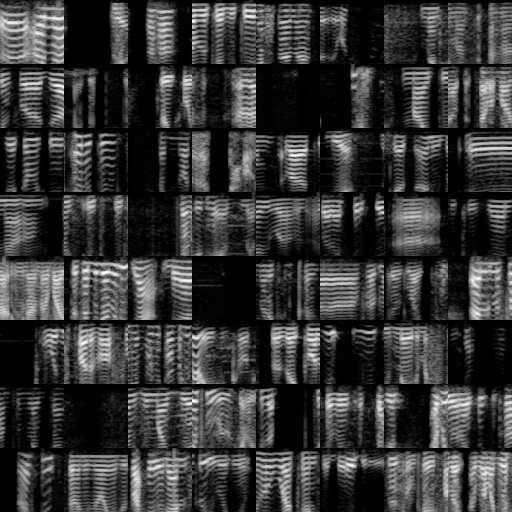
\includegraphics[width=\textwidth]{./fig/samples_groundtruth.png}
        \caption{Real (actual)}
        \label{fig:samples_real}
    \end{subfigure}
    \qquad
    \begin{subfigure}[b]{0.4\textwidth}
        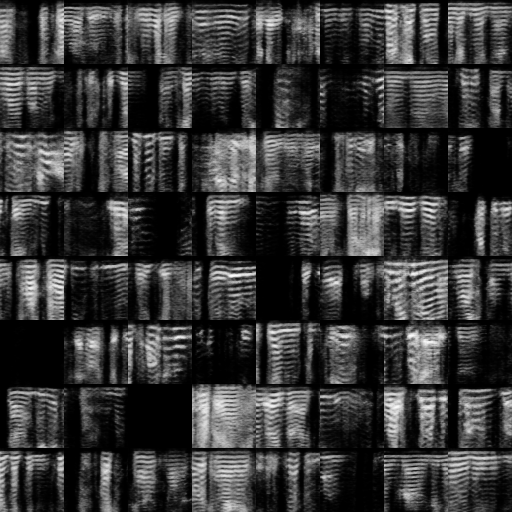
\includegraphics[width=\textwidth]{./fig/samples_5419.png}
        \caption{Fake (generated)}
        \label{fig:samples_fake}
    \end{subfigure}
    \caption{Comparison of real and generated ($\sim$ 5000 generator iterations)
    spectrogram samples from all speakers. Each grid contains 64 samples.}
    \label{fig:samples_comparison}
\end{figure}

\subsection{GAN Adversarial attacks}

Within the GAN framework, we train models for untargeted attacks by using all
data available from speakers that the speaker recognition systems was trained on, 
irrespective of class label. We show that an untargeted model able to generate 
data from the real distribution with enough variety can be used to perform 
adversarial attacks. We provide details in the untargeted attacks 
subsection \ref{sub:untargeted}. Figure~\ref{fig:histogram_untargeted} depicts
that our GAN-trained generator successfully learns all speakers across the
dataset, without mode collapsing.
\begin{figure}[t]
    \centering
    \begin{subfigure}[b]{0.4\textwidth}
        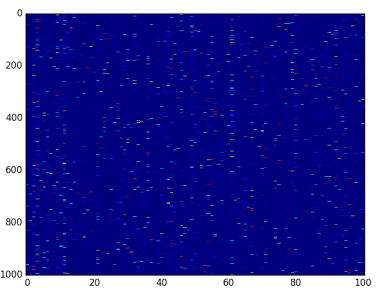
\includegraphics[width=\textwidth]{./fig/conf_mat_untargeted.png}
        \caption{Our speaker classifier's softmax distribution of 1000 samples 
        on approximately 100 speakers.}
        \label{fig:cm_untargeted}
    \end{subfigure}
    \qquad
    \begin{subfigure}[b]{0.4\textwidth}
        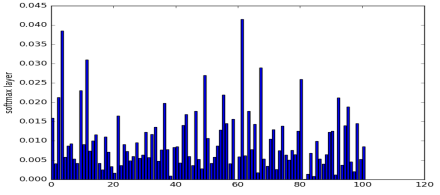
\includegraphics[width=\textwidth]{./fig/histogram_untargeted.png}
        \caption{Our speaker classifier's distribution of randomly sampled 
        speech from the generative model.}
        \label{fig:histogram_untargeted}
    \end{subfigure}
    \caption{Summary of untargeted attacks. Red represents high confidence.}
    \label{fig:histogram_summary}
\end{figure}

The models for targeted attacks can be trained in two manners: 1) 
conditioning the model on additional information, e.g. class labels, as
described in~\cite{mirza2014conditional}; 2) using only data from the label 
of interest. While the first approach might result in mode collapse, a drawback
of the second approach is that the discriminator, and by consequence the
generator, does not have access to universal\footnote{We draw a parallel with 
Universal Background Models in speech.}. properties of speech. In the targeted 
attacks subsection \ref{sub:targeted} we propose a new objective function that allows 
using the data from all speakers.  

\subsubsection{Untargeted attacks}
\label{sub:untargeted}
For each speaker audio data in the test set, we compute a Mel-Spectrogram as
descibred in section \ref{sub:processdata}. The resulting Mel-Spectrogram is
then fed into the CNN recognizer and we extract a 505-dimensional feature $G$ from
the penultimate fully-connected layer (L7) in the pre-trained CNN model
(\ref{fig:CNN}) trained on the train partition of the real speech dataset with all 
speaker IDs.  This deep feature/embedding $G$ is then used to train a 
K-nearest-neighbor (KNN) classifier, with K equal to 5.

To control the generator trained by our WGAN, we feed the generated
Mel-Spectrograms into the same CNN-L2 pipeline to extract their corresponding
feature $\widehat G$. Utilizing the pre-trained KNN, each sample is assigned to
the nearest speaker in the deep feature space. Therefore, we know which speaker
our generated sample belongs to when we attack our CNN recognizer. We evaluate our
controlled WGAN samples against the state-of-the-art CNN recognizer, and the
confusion matrix can be found in Figure \ref{fig:conf_mat_cnn_knn}. Although not
included in the figure, \textbf{neither WaveNet samples nor SampleRNN samples
were able to attack the recognition model in the same way.}~\footnote{Unlike our
method, neither were they successful in attacking a GMM-UBM speaker recognizer.}


\subsubsection{Targeted attacks}
\label{sub:targeted}
However, the most natural attack is one in which we train a GAN to directly fool
a speaker recognition system, i.e., to produce samples that the system
classifies as matching a target speaker with reasonable confidence. We attempted
using data from the target speaker only, but the generated samples did not fool
the speaker recognition systems. To circumvent this, we propose a 
modification to the critic's objective function that allows it to learn to 
differentiate between not only real samples and generated samples, but also between real speech samples from a target 
speaker and real speech samples from other speakers. We do this by adding a term 
to the critic's loss that encourages its discriminator to classify real speech 
samples from untargeted speakers as fake. The critic's loss $L_C$ becomes:
\begin{align}
    \underbrace{\underset{\boldsymbol{\widetilde{x}} \sim \mathbb{P}_{g}}{\mathbb{E}}  \big[D(\boldsymbol{\widetilde{x}})\big]}_\text{Generated Samples} \color{red} + \alpha * \underbrace{\underset{\boldsymbol{\dot{x}} \sim \mathbb{P}_{\dot{x}}}{\mathbb{E}}  \big[D(\boldsymbol{\dot{x}})\big]}_\text{Different Speakers} \color{black} - \underbrace{\underset{\boldsymbol{x} \sim \mathbb{P}_{r}}{\mathbb{E}}  \big[D(\boldsymbol{x})\big]}_\text{Real Speaker}  + \underbrace{\lambda \underset{\boldsymbol{\hat{x}} \sim \mathbb{P}_{\hat{x}}}{\mathbb{E}}  \big[(\lVert \nabla_{\boldsymbol{\hat{x}}} D(\boldsymbol{\hat{x}}) \rVert_2 - 1)^2\big]}_\text{Gradient Penalty}
\end{align}
where $P_{\hat{x}}$ is the distribution of samples from other speakers, and
$\alpha$ is a tunable scaling factor. In our experiments, we trained this GAN
with 1 target speaker and a set of over 100 'other' speakers. On each critic
iteration, we would feed it with a batch of samples from one target speaker, 
and a batch of data uniformly sampled from the other speakers. During training 
we used two approaches. The first one used an $\alpha$ of 0.1 (we found that not 
including this scaling factor led to serious overfitting and poor convergence of 
the GAN). The second one used an $\alpha$ of 1 combined with modifications to 
the network parameters, including different weight initialization, learning
rates and addition of gaussian noise to the target speaker data. We invite
readers to our github repo for details. Results are demonstrated in Figure
\ref{fig:confusion_matrices}: the confusion matrices in ~\ref{fig:conf_mat_cnn} 
and ~\ref{fig:conf_mat_cnn_spk0} show that all energy is concentrated in the
targeted speaker ids, 1 and 0 respectively.
\begin{figure}[t]
    \centering
    \begin{subfigure}[b]{0.3\textwidth}
        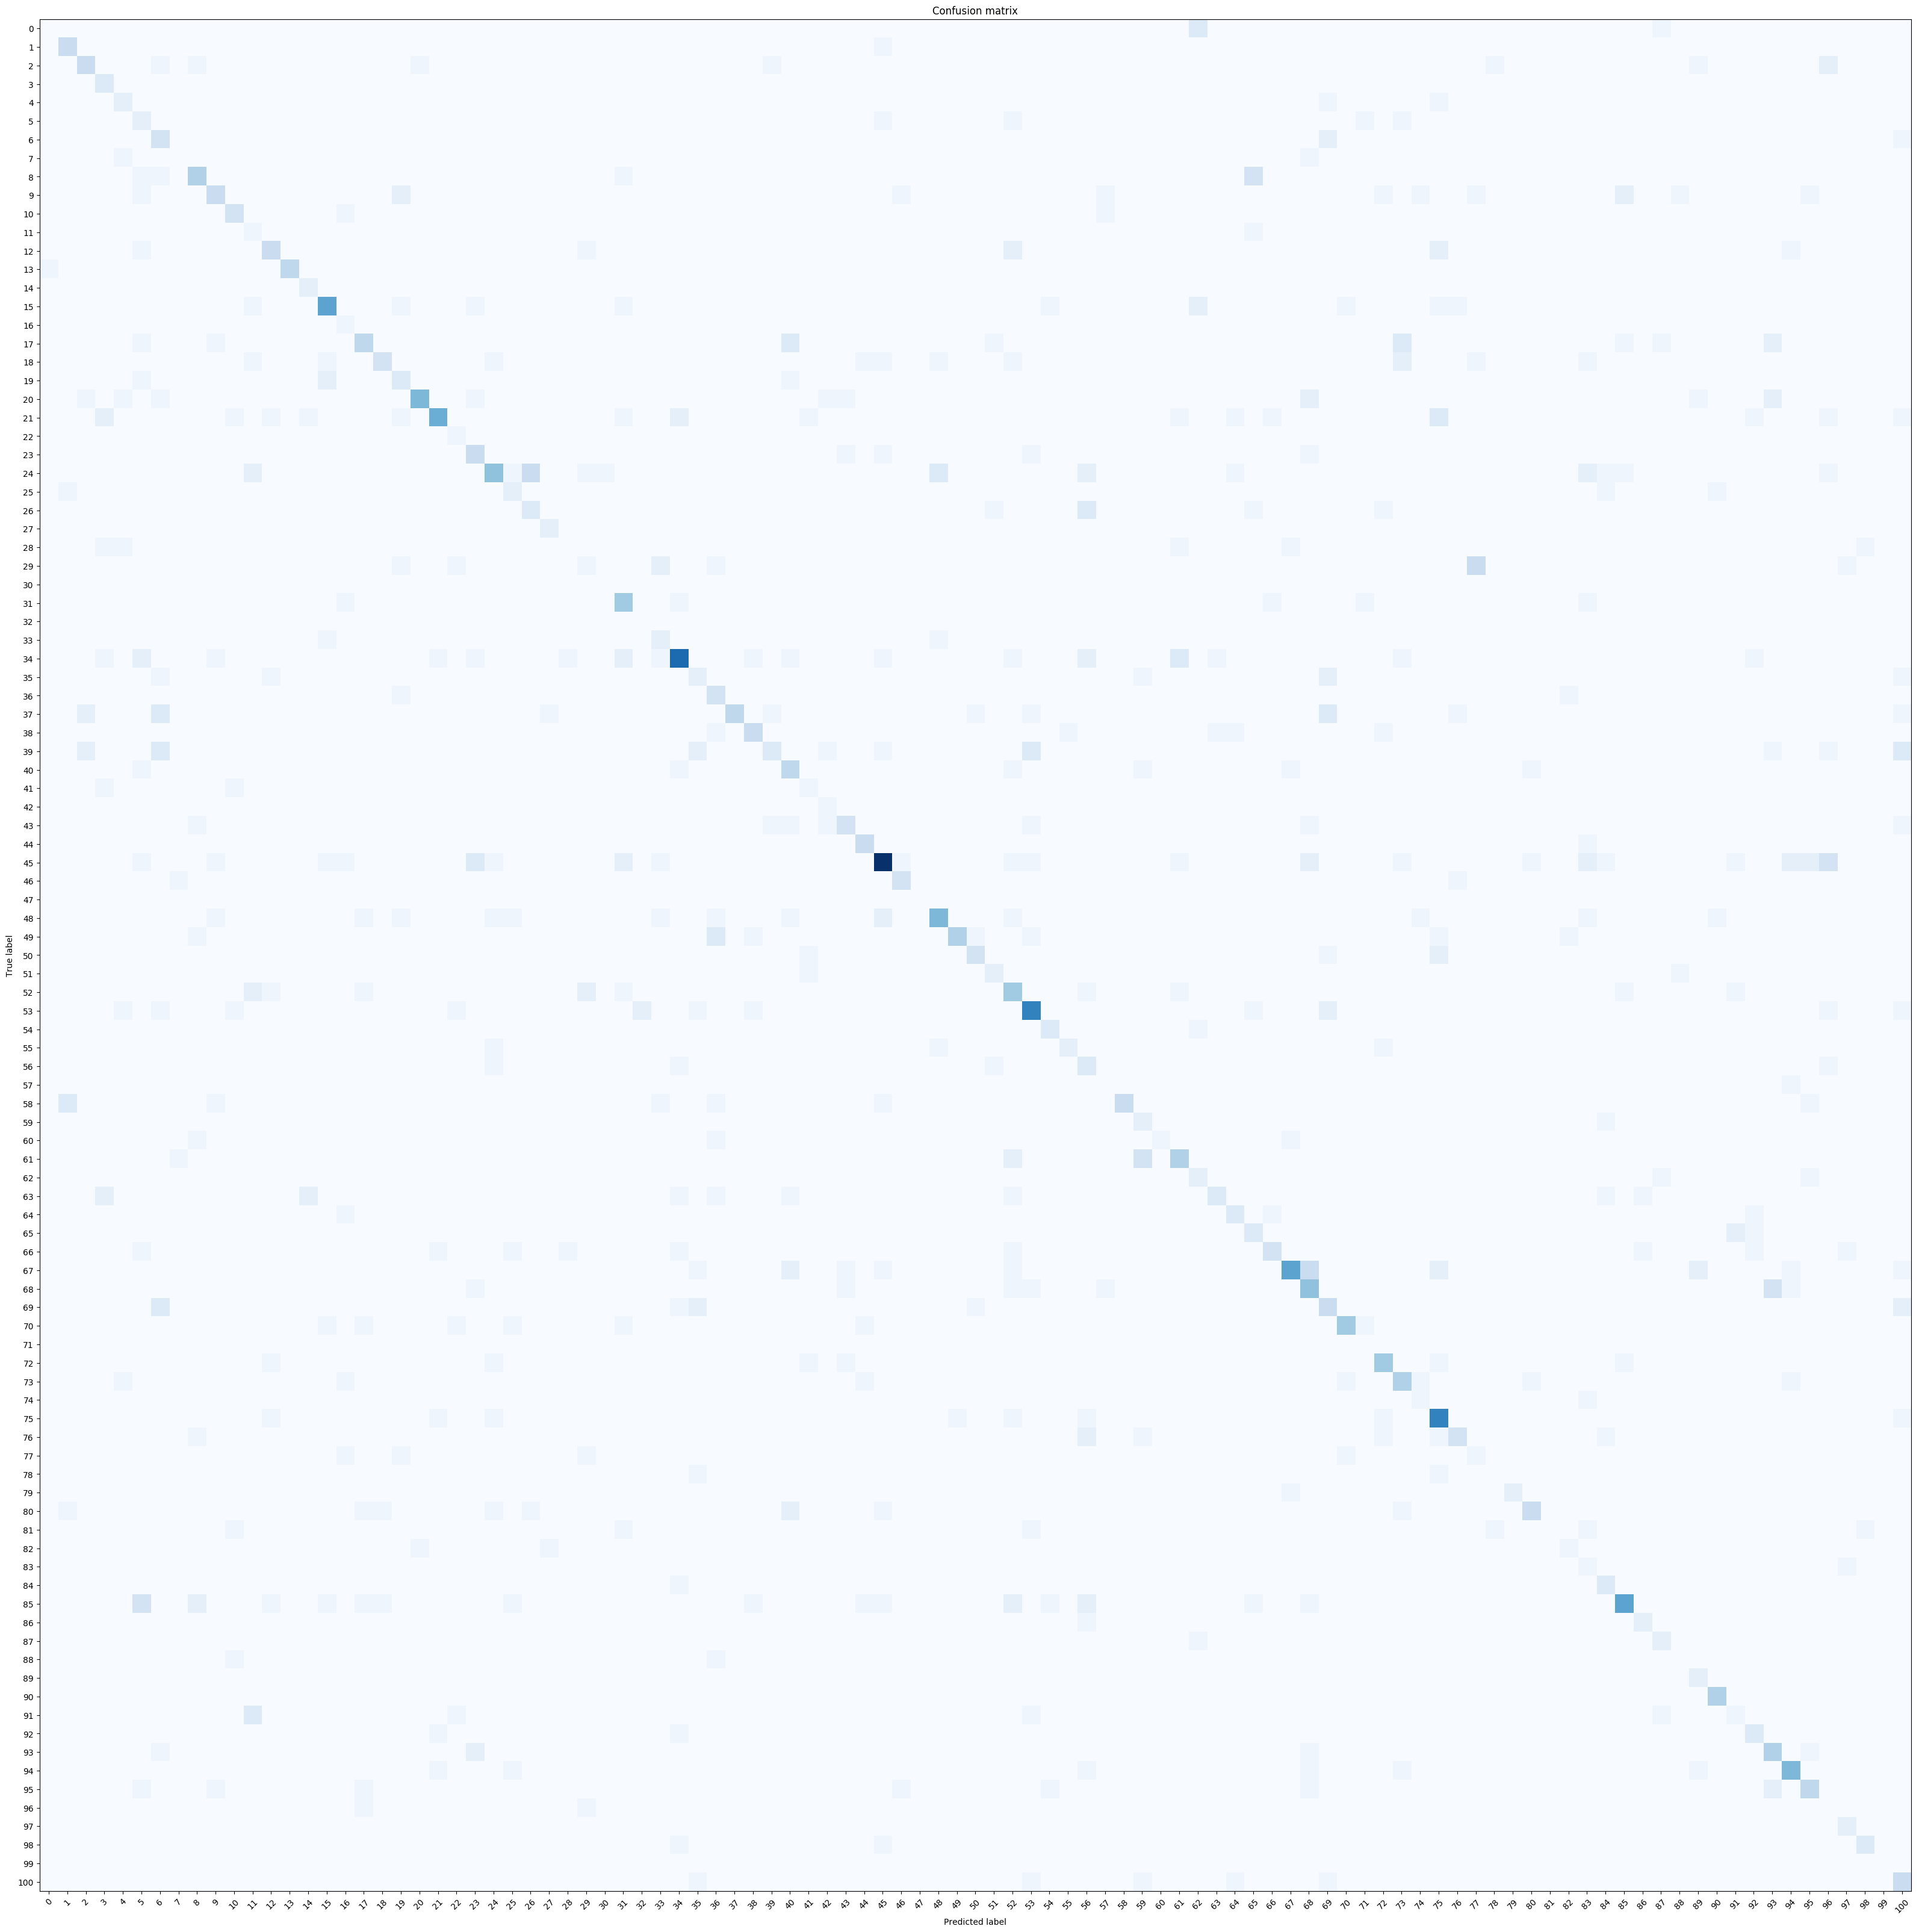
\includegraphics[width=\textwidth]{./fig/conf_mat_cnn_knn.png}
        \caption{Confusion matrix of \\untargeted model}
        \label{fig:conf_mat_cnn_knn}
    \end{subfigure}
    \quad
    \begin{subfigure}[b]{0.3\textwidth}
        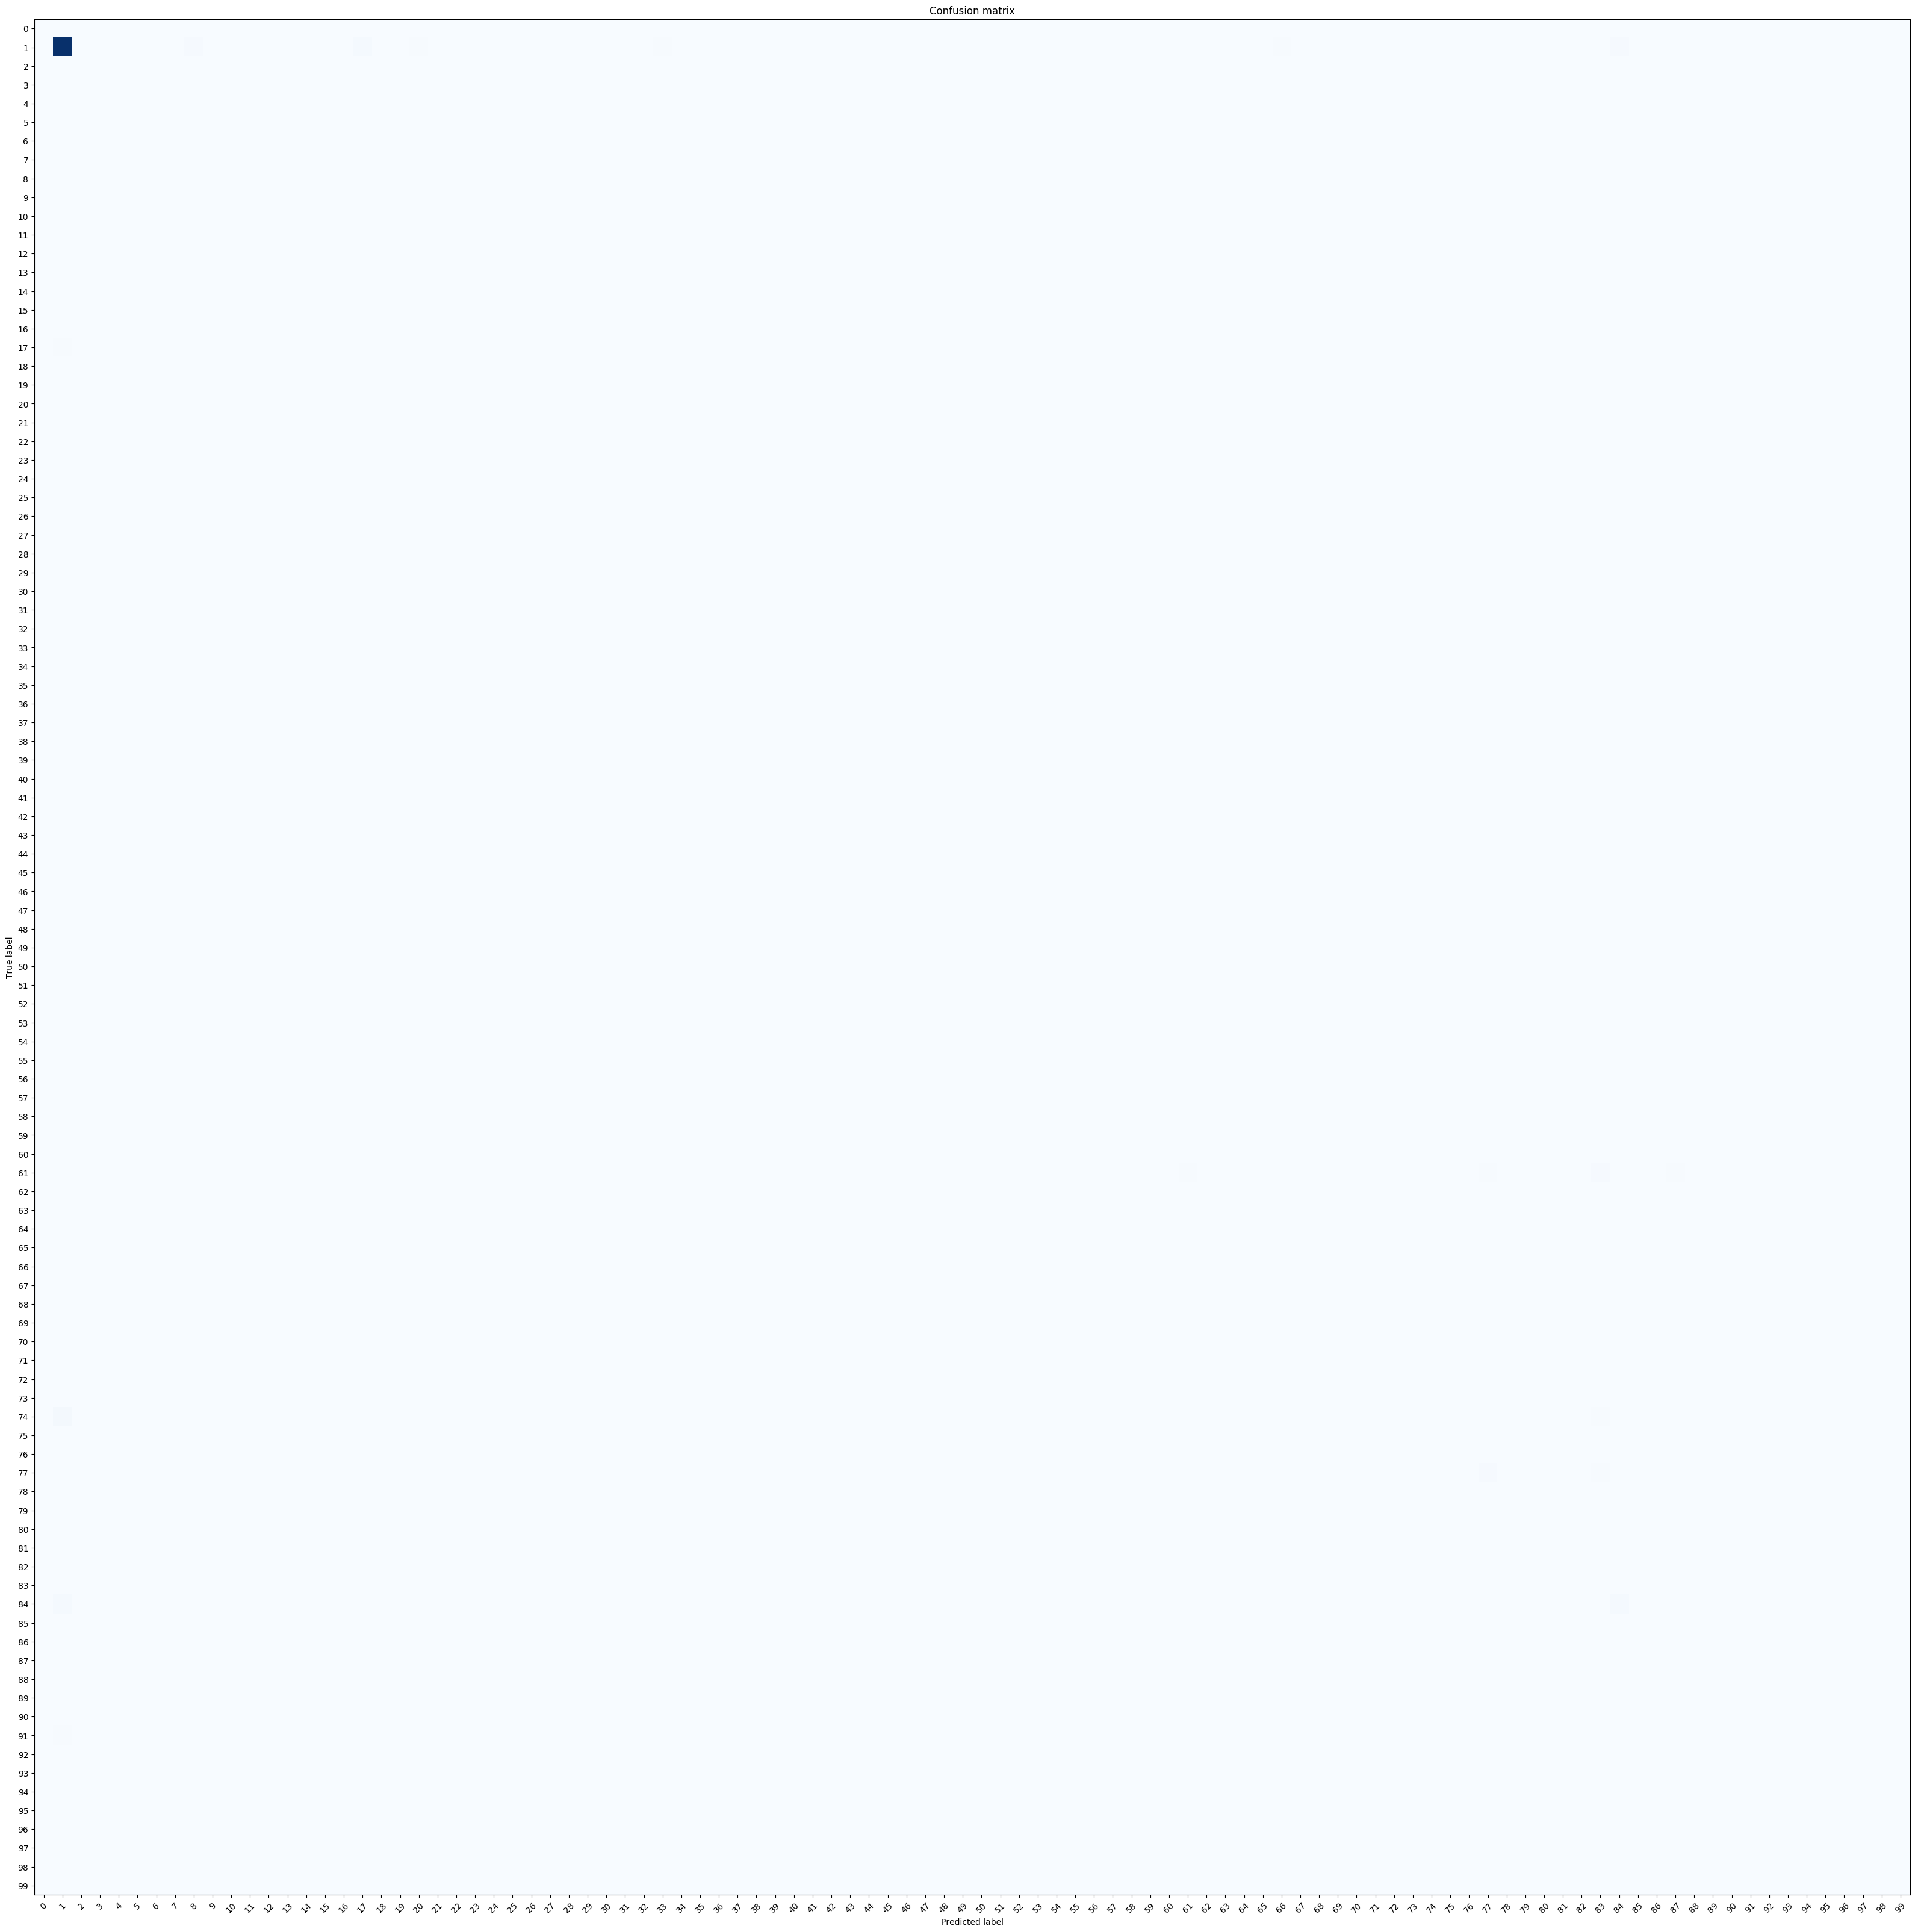
\includegraphics[width=\textwidth]{./fig/conf_mat_cnn_knn_targeted.png}
        \caption{Confusion matrix of targeted attacks with $\alpha = 0.1$}
        \label{fig:conf_mat_cnn}
    \end{subfigure}
    \quad
    \begin{subfigure}[b]{0.3\textwidth}
        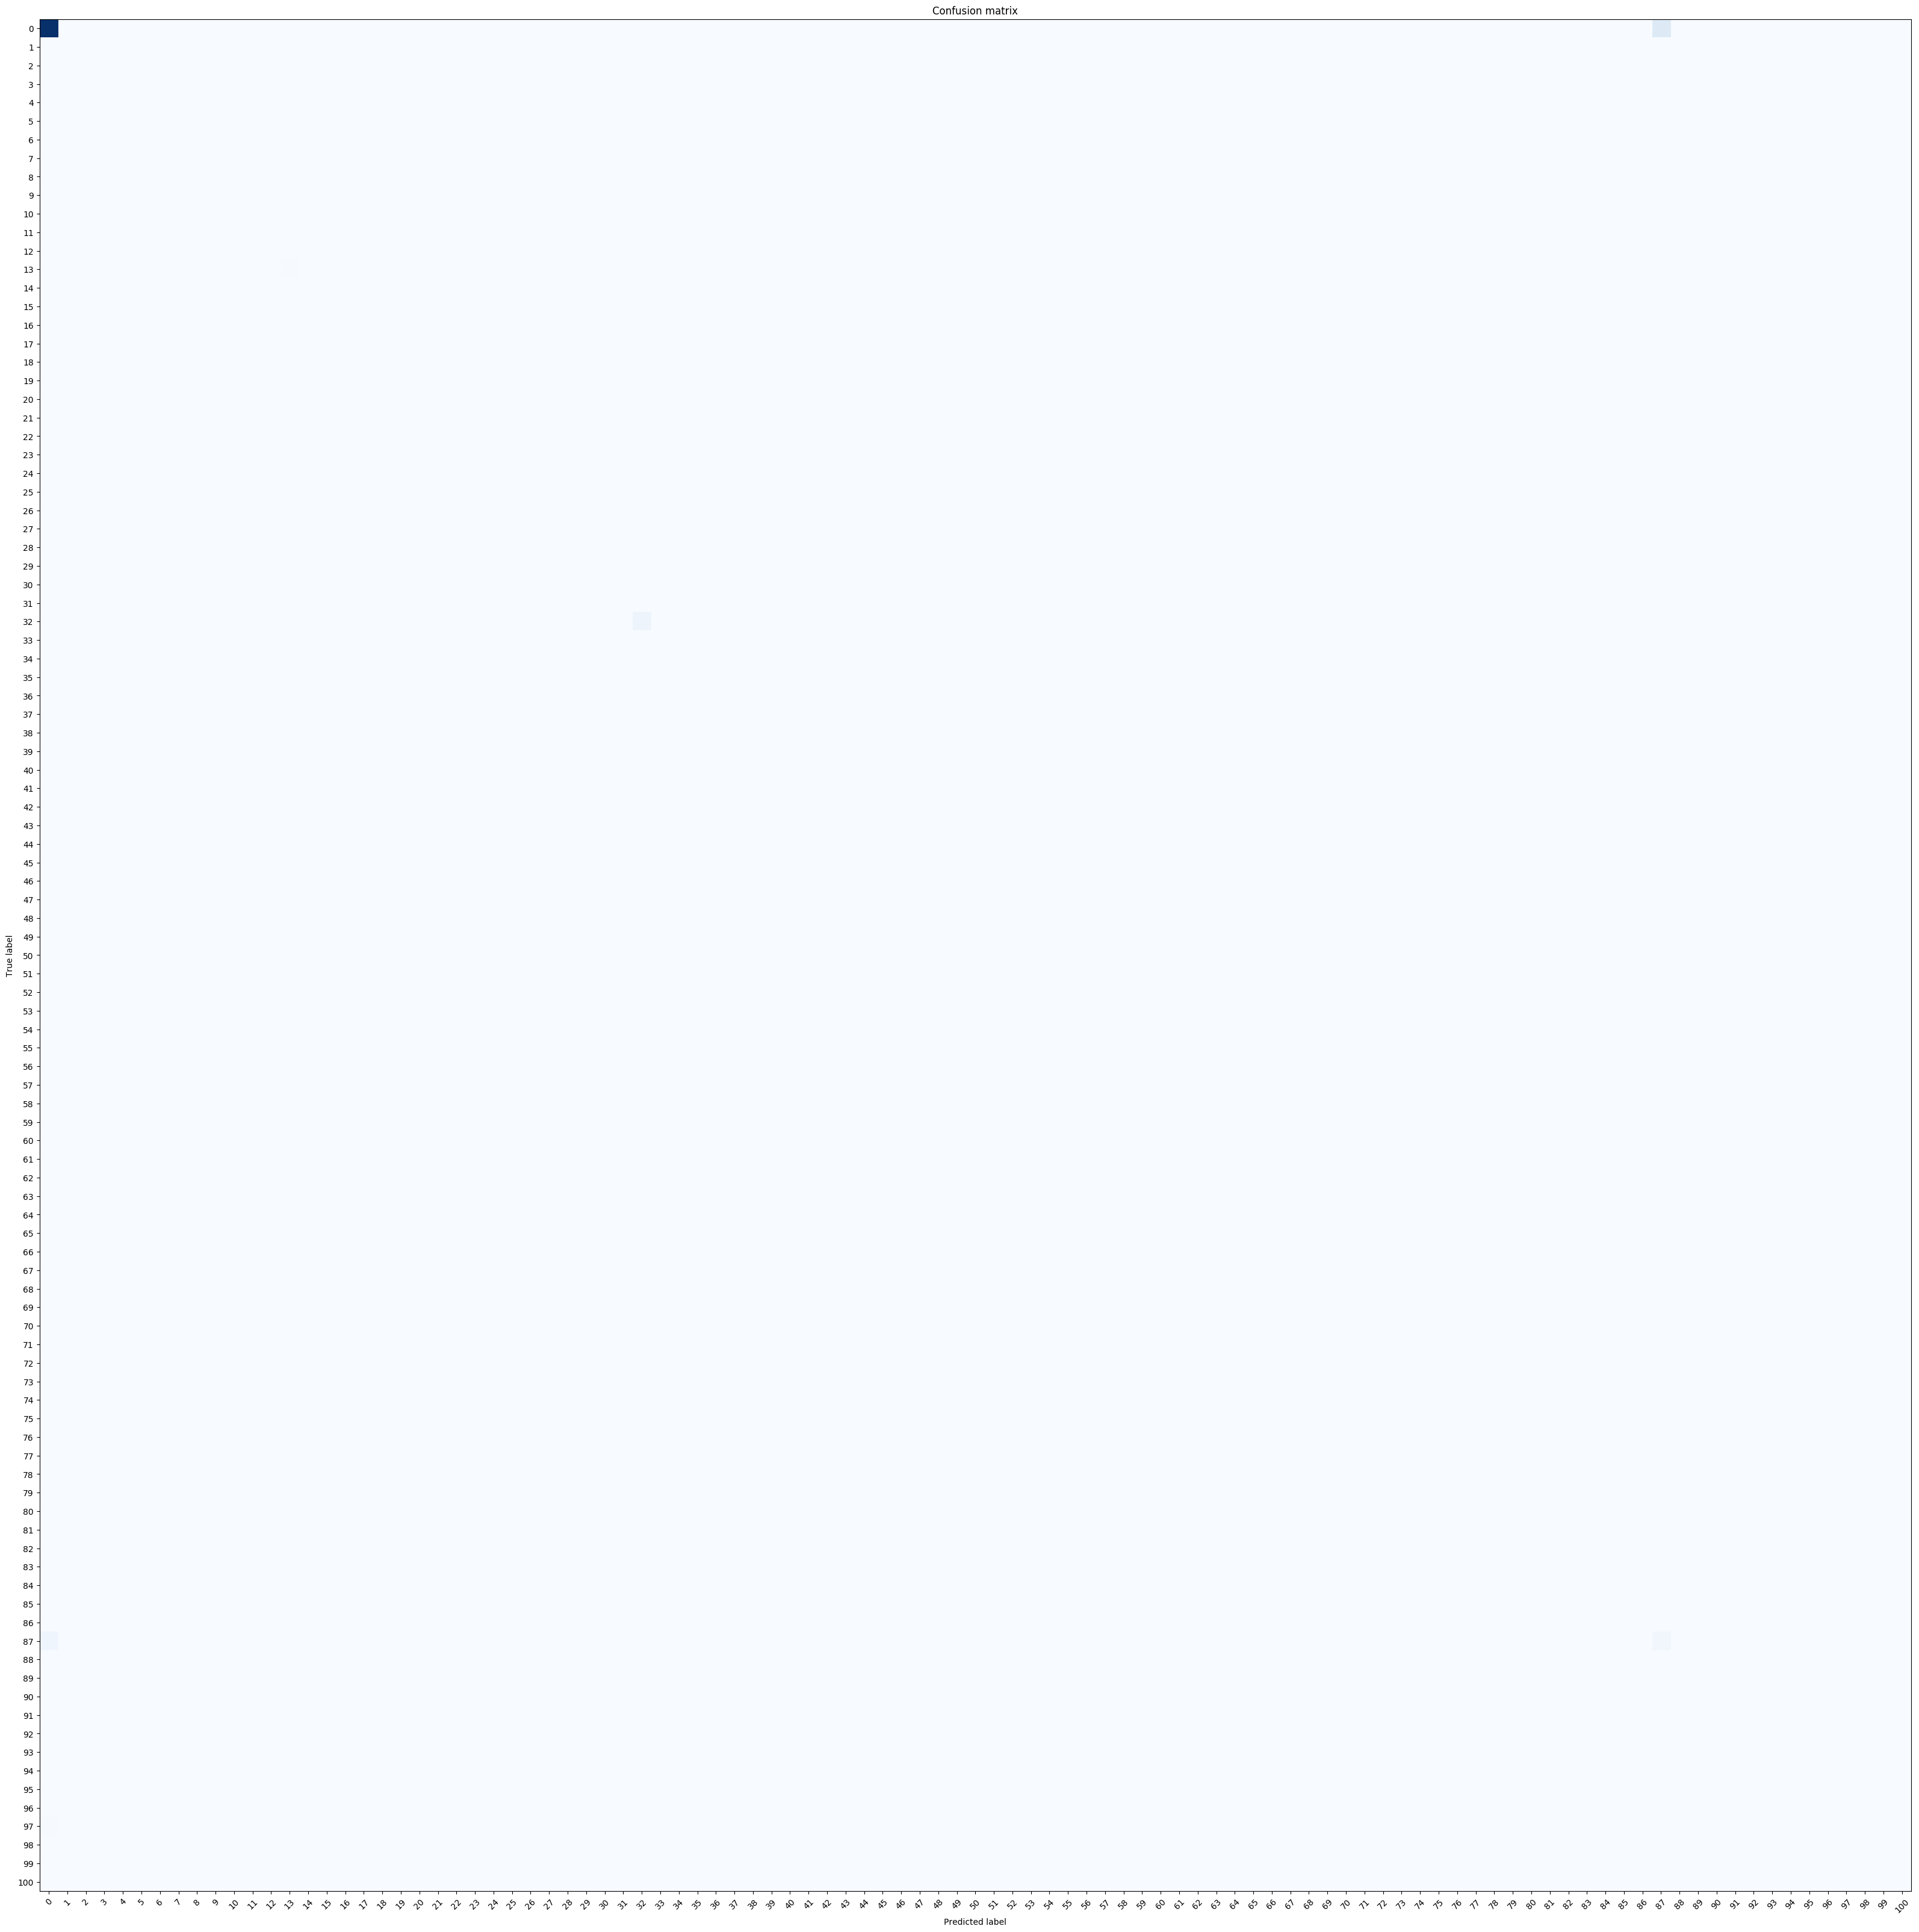
\includegraphics[width=\textwidth]{./fig/conf_mat_cnn_knn_spk0.png}
        \caption{Confusion matrix of targeted attacks with $\alpha = 1$}
        \label{fig:conf_mat_cnn_spk0}
    \end{subfigure}
    \caption{Confusion matrix of targeted attacks}
    \label{fig:confusion_matrices}
\end{figure}
